 \documentclass[conference]{IEEEtran}\usepackage[]{graphicx}\usepackage[]{color}
%% maxwidth is the original width if it is less than linewidth
%% otherwise use linewidth (to make sure the graphics do not exceed the margin)
\makeatletter
\def\maxwidth{ %
  \ifdim\Gin@nat@width>\linewidth
    \linewidth
  \else
    \Gin@nat@width
  \fi
}
\makeatother

\definecolor{fgcolor}{rgb}{0.345, 0.345, 0.345}
\newcommand{\hlnum}[1]{\textcolor[rgb]{0.686,0.059,0.569}{#1}}%
\newcommand{\hlstr}[1]{\textcolor[rgb]{0.192,0.494,0.8}{#1}}%
\newcommand{\hlcom}[1]{\textcolor[rgb]{0.678,0.584,0.686}{\textit{#1}}}%
\newcommand{\hlopt}[1]{\textcolor[rgb]{0,0,0}{#1}}%
\newcommand{\hlstd}[1]{\textcolor[rgb]{0.345,0.345,0.345}{#1}}%
\newcommand{\hlkwa}[1]{\textcolor[rgb]{0.161,0.373,0.58}{\textbf{#1}}}%
\newcommand{\hlkwb}[1]{\textcolor[rgb]{0.69,0.353,0.396}{#1}}%
\newcommand{\hlkwc}[1]{\textcolor[rgb]{0.333,0.667,0.333}{#1}}%
\newcommand{\hlkwd}[1]{\textcolor[rgb]{0.737,0.353,0.396}{\textbf{#1}}}%
\let\hlipl\hlkwb

\usepackage{framed}
\makeatletter
\newenvironment{kframe}{%
 \def\at@end@of@kframe{}%
 \ifinner\ifhmode%
  \def\at@end@of@kframe{\end{minipage}}%
  \begin{minipage}{\columnwidth}%
 \fi\fi%
 \def\FrameCommand##1{\hskip\@totalleftmargin \hskip-\fboxsep
 \colorbox{shadecolor}{##1}\hskip-\fboxsep
     % There is no \\@totalrightmargin, so:
     \hskip-\linewidth \hskip-\@totalleftmargin \hskip\columnwidth}%
 \MakeFramed {\advance\hsize-\width
   \@totalleftmargin\z@ \linewidth\hsize
   \@setminipage}}%
 {\par\unskip\endMakeFramed%
 \at@end@of@kframe}
\makeatother

\definecolor{shadecolor}{rgb}{.97, .97, .97}
\definecolor{messagecolor}{rgb}{0, 0, 0}
\definecolor{warningcolor}{rgb}{1, 0, 1}
\definecolor{errorcolor}{rgb}{1, 0, 0}
\newenvironment{knitrout}{}{} % an empty environment to be redefined in TeX

\usepackage{alltt}
\pagestyle{plain}
\usepackage[cmex10]{amsmath}
\usepackage{multirow}
%\usepackage{caption} 
%\captionsetup[table]{skip=3pt}

\hyphenation{op-tical net-works semi-conduc-tor}
\IfFileExists{upquote.sty}{\usepackage{upquote}}{}
\begin{document}

\title{Evading stepping stone detection by using enough chaff}
%Evaluation of passiv stepping stone detection techniques under chaff and delay}


\author{\IEEEauthorblockN{Michael Shell}
\IEEEauthorblockA{Georgia Institute of Technology\\
someemail@somedomain.com}
\and
\IEEEauthorblockN{Homer Simpson}
\IEEEauthorblockA{Twentieth Century Fox\\
homer@thesimpsons.com}
\and
\IEEEauthorblockN{James Kirk\\ and Montgomery Scott}
\IEEEauthorblockA{Starfleet Academy\\
someemail@somedomain.com}}


\IEEEoverridecommandlockouts
\makeatletter\def\@IEEEpubidpullup{6.5\baselineskip}\makeatother
\IEEEpubid{\parbox{\columnwidth}{
    Network and Distributed Systems Security (NDSS) Symposium 2020\\
    23-26 February 2020, San Diego, CA, USA\\
    ISBN 1-891562-61-4\\
    https://dx.doi.org/10.14722/ndss.2020.23xxx\\
    www.ndss-symposium.org
}
\hspace{\columnsep}\makebox[\columnwidth]{}}


\maketitle          

\begin{abstract}

Bla
\end{abstract}



\section{Introduction}

%\textcolor{red}{Network attackers frequently use a chain of compromised intermediate nodes to attack a target machine and maintain anonymity. This chain of nodes between the attacker and the target is calleda stepping stone chain. }


Malicious actors on the Internet frequently use chains of compromised hosts to relay their attack, in order to obtain access to restricted resources and to reduce the chance of being detected. These hosts, called \textbf{stepping-stones}, are used by the attacker as relay machines, to which they maintain access using tools such as SSH or telnet \textcolor{red}{reference}. 

Accessing a server via multiple relayed TCP connections can make it harder to tell the intruder's geographical location, and enables attackers to hide behind a long interactive stepping-stone chain. Furthermore, it is often required to relay an attack via privileged hosts in a network that have access to restricted resources. 

However, detecting that a host is used in a stepping-stone chain is a clear indication of malicious behaviour. If a stepping-stone intrusion can be detected during the attack stage, the connection can be terminated to interrupt the attack. Stepping-stone detection (SSD) primarily looks at network traffic, with many approaches aiming to identify potential correlation between two connections going from or to a particular host. To hide correlation between relayed packets, intruders can impose delays on packet transfer and inject additional \textit{chaff} packets into the connections.

There are a number of approaches to detect stepping-stones, with the earliest one having been proposed by Zhang and Paxson in 2000 \textcolor{red}{citation needed?}. However like many intrusion attacks, stepping-stones are rare and there exists no public data representing real stepping-stone behaviour, and researchers have to rely on synthetic data. Some attempts have been made to create publicly available stepping-stone testbeds, but most researchers evaluate their SSD methods on self-provided data. The underlying generating implementations often differ significantly, which makes their direct comparison of the achieved results impossible. Additionally, we find that implemented evasive behaviours are often too simplistic and thus increase detection rates. 

In this work, we provide an independent framework to generate data representing stepping-stone behaviour ....
We use this data to provide an in-depth evaluation of current passive SSD methods and compare their results. Furthermore, we show that by inserting enough chaff perturbations in the right form, an intruder can evade all current SSD methods successfully


\section{Background}

When a person logs into one computer and from there logs into another computer and so on, we refer to the sequence of logins as a connection chain[18]. 
In an interactive stepping-stone attack, an attacker located at the origin host, which we call \textit{host O} sends commands to and awaits their response from a target, \textit{host T}, typically by using terminal emulation programs like TelNet or SSH. These commands and responses are proxied via a chain of one or more intermediary hosts, the stepping-stones, which we call \textit{host} $S_1$, \dots, $S_N$, such as depicted in Fig. \textcolor{red}{insert image}. 

Stepping-stone detection (SSD) is a process of observing all incoming and outgoing connections in a network and determining which ones are parts of a connection chain. %This problem is closely related to the problem of tracing intruders through the Internet by following the connection chain. 
SSD typically either aims at classifying a host as a stepping stone if two connections involving this host appear to be correlated, or at classifying a connection as part of a chain if its behaviour differs from regular connections. In addition, several SSD methods aim to estimate the overall length of the stepping-stone chain to help tracing the intruder by following the connection chain. 
A traffic collection sensor is typically placed in the vicinity of the examined host to provide the necessary data. 

\textcolor{red}{insert citation} identify another form of stepping-stones called \textit{store-and-forward}, which transfer data within files in a non-interactive manner. Though harder to detect than interactive connections, this procedure limits the attackers ability to explore the target, which is why SSD research has been primarily concerned with interactive stepping-stones.

\subsection{Packet delays}

\subsection{Chaff perturbations}



\section{Related work}\label{Sec:Relatedwork}

\subsubsection{Evasion tactics}

Padhye et al. \cite{padhye2010evading} in 2010 have proposed a packet buffering method to decorrelate packets in the input flow from the output flow. Using this technique and enough chaff packets, the authors generate a constant-rate flow that resembles multimedia streams such as Voice over IP. However, the authors only test their framework against watermark-based SSD methods. 

Yang et al. \cite{yang2018sniffing} have recently 

\subsection{Datasets}


In 2006, Xin et al. \cite{xin2006testbed} developed a standard test bed for stepping-stone detection, called \textit{SST}. 
The main objectives in the development of SST were to enable a reproducible evaluation of stepping stone chain detection algorithms with easy configuration, management and operation. The tool allows for an arbitrary number of intermediate hosts and generates scripts to mimic interactive SSH and TelNet connections. 
To insert time delays and chaff perturbations, the authors modified the OpenSSH protocol on the intermediary hosts. Delays can be drawn from a uniform distribution while chaff can be drawn from a Poisson or Pareto distribution. To our knowledge, SST has only been used for evaluation by Zhang et al. \cite{zhang2005stepping}, and is not available anymore. \textcolor{red}{say something why evasion not sufficiently implemented}

Another approach to use publicly available data comes from Houmansadr et al. \textcolor{red}{insert citations}. The authors use the well-known CAIDA 2016 anonymized data traces \textcolor{red}{insert citation} to evaulate different watermarking methods for SSD. To simulate stepping stone behaviour, packet delays and drops are imposed retroactively on selected connections using Laplace and Bernoulli distributions with different rates. While this procedure seems sufficient for the evaluation of watermarking methods, it falls short on simulating an actual connection chain and leaves out chaff perturbations. 


Wang et al. \cite{wang2018research} recently conducted an extensive survey of  stepping stone intrusion detection. The authors group methods according to the respective methodology into 
\begin{itemize}
\item content-thumbprint,
\item time-thumbprint,
\item packet counting,
\item random-walk-based,
\item cross-over packet-based,
\item watermarking,
\item network-based,
\item and software-defined-networking-based, 
\end{itemize} 
but do not cover \textcolor{red}{graph-based methods} such as \cite{gamarra2018analysis} %or \cite{apruzzese2017detection}, 
or anomaly-based methods such as \cite{di2011detecting}, which are increasing in popularity recently.
The authors then proceed to explain the different methods and highlight their benefits and shortcomings. The authors discuss open problems, but do not provide a comparison of detection rates. 

Shullich et al. \cite{shullich2011survey} in 2011 also conducted a survey on stepping stone intrusion detection. The authors perform a similar grouping of methods, but also discuss related work in evasion tactics and test frameworks. The authors furthermore give an outlook on areas for future research, such as hacker motivation, the cardinality problem when correlating connection pairs, the difficulty of tracing back chains through firewalls, the lack of real-world data examples, or detection in covert channels or protocols such as UDP.  

\cite{almulhem2007survey}

Stepping Stone Detection Techniques: Classification and State-of-the-Art, bad though

Metrics: A Study on the Performance Metrics forEvaluating Stepping Stone Detection (SSD)
Stepping Stone Detection: Measuring the SSD Capability


\section{Dataset creation}\label{Sec:Datasetcreation}

Our goal is to simulate data that reflects the different aspects of interactive stepping-stone behaviour in a reproducable manner. For a fair and thorough evaluation, we want to cover different settings and interactions to incorporate enough variation in the data to highlight strengths and weaknesses of different SSD methods. Furthermore, we need to generate sufficient data to effectively train some of the included methods. 

In order to consider all these factors, we rely on the virtualisation framework Docker. Docker enables us to script the repeated creation of steppings-stone chains within a virtual network in a scalable manner. \textcolor{red}{while allowing network different settings}. 

\textcolor{red}{write about Docker advantages in terms of speed and controllability}

\subsection{Simulating stepping stones with SSH-tunnels and Docker}\label{Sec:Setup}

We want to capture data not only from one interaction in a fixed stepping-stone chain, but from many interactions and chains with different settings. For that, we run multiple simulations, with each simulation establishing a stepping-stone chain and controlling the interactions between host O and host T. A simulation and the corresponding traffic capture is \textit{red}{described} a capture-script. 

A simulation begins with the start-up of the necessary containers and ends with their takedown. We represent host O, host T, and host $S_1,\dots,S_n$ with SSH-daemon containers.  To establish a connection chain, we connect these containers via SSH-tunnels, with the first tunnel forwarding the required port from host O to host $S_1$, which is then forwarded to host $S_2$ by the second tunnel etc. One benefit of SSH-tunnels from an attackers perspective is that they do not just simply forward packets, but act as independent encrypted TCP-connections along with independent packet confirmations.  Fig. \textcolor{red}{...} depicts a packet transfer via an exemplary chain. 

Traffic is captured both at host T and host $S_n$, which acts as the final stepping-stone in the chain and is most likely the target of a detection algorithm. 




%insert figure with one and with three stepping stones



%SSH tunnel on respective port on the starting point of the chain, tunnels to port on the next point in the chain. Finally, Refer to figure. 

\subsection{Simulating interactive SSH-traffic}\label{Sec:Simulating_interactive}

In order to generate enough data instances representing interactive stepping stone behaviour, we automatised the communication between host O and host T.  For each simulation, we generate a script which passes SSH-commands from host O to host T.

For script-based session creation, several measures have been taken to make them realistic. First, each session tries to mimic a real user's action. We compiled a command database which consists of common commands and their usage frequency, similar to \cite{xin2006testbed}.% \cite{rossey2002lariat}. 
Commands are drawn randomly according to their usage frequency and concatenated to a script. 
Commands can either be atomic, such as "ls-la" or "pwd", or compound. Compound commands need additional input such as the directory and name of a specific file that is transferred or input text for a \textcolor{red}{....}. The content and sometimes length of these inputs as well as transferred files are randomised appropriately when a compound command is drawn. 

To simulate human behaviour that is reacting to the response from host T, all commands are separating by \textit{sleep}-commands for time $t$, which is drawn from a Cauchy-distribution. By using a Cauchy-distribution, we allow for a small number of large $t$-values that simulate longer thinking periods.  


Scripts are of varying length and end once the \textit{End}-command is drawn from the command catalogue. 

\textcolor{red}{show exemplary script}.

%To do so, we generate a script with SSH-commands at the start of each \textcolor{red}{execution} that is passed and run by the \textcolor{red}{starting point} of the chain. The generated script consists of a sequence of ordinary SSH-commands \textcolor{red}{list them here?}, which are drawn randomly from a command catalogue and are each separated by \textit{sleep}-commands for a time $t$ that is drawn each time from a Cauchy-distribution. The average sleep-time is around \textcolor{red}{insert}. The length of the script is reached when the \textit{end}-command is drawn from the catalogue.
%To evaluate the stepping stone detection capabilities of different proposed methods, we created a \textcolor{red}{realistic dataset...}
%\textcolor{red}{Insert example}

%For script-based session creation, several measures havebeen taken to make them realistic. First, each session tries tomimic a real user’s action. All users of the scripts are real useraccounts in the clients. The users are divided into four groups:administrators, secretaries, programmers, and researchers. For each type of user, there is large command database which con-sists of the common commands and their historic frequency ofexp_version -exit 5.0if {$argc!=1} {send_user "usage: ftp-rfc \[#] \[-index]\n"exit}set file "rfc$argv.Z"set timeout 60spawn ftp ftp.uu.netexpect "Name*:"send "anonymous\r"expect "Password:"send "expect@nist.gov\r"expect "ftp>"send "binary\r"expect "ftp>"send "cd inet/rfc\r"expect "550*ftp>" exit "250*ftp>"send "get $file\r"expect "550*ftp>" exit "200*226*ftp>"closewaitsend_user "\nuncompressing file - wait...\n"exec uncompress $fileFig. 7.  Example script for a TELNET session
%use [22]. A portion of the command database for programmersare shown in Table I. Each Expect script is associated witha user, and the commands within the script are drawn fromcorresponding database according to their frequency. Thereare two types of commands: atomic and compound. Atomiccommands only need the user type the command line andthe system will parse the command and print the output.Examples are “ls -la”, “pwd”. Compound commands requiremore interaction. A simple example is “mail xxxx”. After theuser enters “mail xxxx” and “Enter” key, the system promptsthe user to enter “subject”, content and “cc” field of the email.Second, the human typing simulation feature of Expect is usedfor all commands of users. Third, more than 50 human actorsfrom four classes were invited to our lab to generate certainstepping stone chains that were recorded by autoExpect.



\subsubsection{Adding network congestion}\label{Sec:congestion}

Hosts in a stepping-stone chains can be separated by varying distances. Some may sit in the same LAN, while others may communicate via the Internet from distant geographical locations. The type of separation between two hosts influences the round-trip-time, bandwidth, and network reliability. 

Docker communication takes place over virtual bridge networks, so the throughput is far higher and more reliable than in real-world networks. %This level of speed and consistency is worrying for our purposes as packet timings will be largely identical on repeated runs of a scenario and any collected data could be overly homogeneous.
To retard the quality of the Docker network to realistic levels, we rely on the emulation tool Netem. Netem \textcolor{red}{add reference} is a Linux command line tool that allows users to artificially simulate network conditions such as high latency, low bandwidth, or packet corruption/drop in a flexible manner.

We apply Netem commands to the network interface of each container, which adds correlated delays to incoming and outgoing packets that are drawn from a normal distribution with mean $\mu$, variance $\sigma^2$, and correlation $\rho_1$. We furthermore apply correlated packet loss and corruption drawn from a binomial distribution with probability $p$ and correlation $\rho_2$. Lastly, we apply an overall limit $B$ on the bandwidth of containers container network interfaces.
 \textcolor{red}{bandwith limiting}.

To allow for different types of host separation, we set the network settings and bandwidth limit for each host container individually before each simulation, and draw each of the given parameters from a suitable distribution. This allows for some hosts to experience very fast and reliable communication while others experience more congested network communication.  \textcolor{red}{(should I specify which one for each? Seems a bit much...)} %before each \textcolor{red}{run} to allow for a good amount of variation in the generated data.
We store the set parameters along with the collected traffic for each simulation to include the effect of network congestion in the evaluation. 

%providing us with the flexibility to set each container's network settings uniquely. 




%This script randomizes the values of each parameter, such as packet drop rate, bandwidth limit, latency, ensuring that every run of a scenario has some degree of network randomization if desired.



\subsubsection{Adding delays}\label{Sec:delays_desc}

To increase detection difficulty as suggested by  \cite{padhye2010evading}, we add transfer delays to packets forwarded by stepping stone hosts. This method, often called \textit{jittering}, can destroy time-based watermarks in packet flows and help decrease observable correlation between two connections. 

We add transfer delays to forward packets again by using NetEm. We draw delays for departing packets on a hosts from a uniform distribution, as suggested by \textcolor{red}{add reference}, covering the interval $[0,\delta_d]$, with zero packet correlation. The value of $\delta_d$ is fixed before each simulation and can be varied to allow for different degrees of packet jittering. 

\textcolor{red}{insert citation} suggested to use long packet delays to decrease decorrelation between packet streams. However, this often leads to difficulties in the TCP-protocol due to the significant increase of packet reordering and response time-outs. We therefore set the maximum value for  $\delta_d$  at $1s$. As we will see in Section \textcolor{red}{...}, this is enough to render watermarking methods obsolete while flow decorrelation can be achieved more effectively by using chaff perturbations. 





\subsubsection{Adding chaff perturbation}\label{Sec:chaff_desc}

We furthermore insert chaff packets to individual connections in the chain to increase detection difficulty \textcolor{red}{citation?}. These chaff packets do not contain actual information and act as noise to decorrelate connections in the chain. To add and filter out packets in a connection, we add additional ports in each SSH-tunnel that are not forwarded through the entire chain.
We then use a NetCat client containers to send and receive packets on these additional ports in both directions. Figure \textcolor{red}{...} depicts this setup. 

%\textcolor{red}{add reference} to send data to both ports from either direction and collect it at the other side. 
The data sent by the client $i$ consists of strings with random size $x$ drawn from a Cauchy-distribution with mean $xx_i$, and is sent in intervals of random length $\delta_c$ drawn from a truncated \textcolor{red}{paretonormal} distribution with mean $yy_i$. Huang et al. \cite{huang2011detecting} have pointed out that packet interarrivals in benign connections often follow a paretonormal distribution, so it seems to be a good choice to make the inserted chaff appear as benign traffic. By adjusting $yy_i$, we can control the rate of chaff sent. \textcolor{red}{explain more}



%\subsection{HTTP-interactions}
 
%In order to provide an additional, different type of interaction between the \textcolor{red}{starting point} and \textcolor{red}{end point}, we directed HTTP traffic over the stepping stone chain. Here, the starting point hosts Scrapy, a web crawling service \textcolor{red}{insert citation}, that surfs the 1 million most popular website by clicking links on them. The requests are sent over the stepping stone chain to the web. 

%This type of traffic is not meant to necessarily represent realistic stepping stone behaviour, but to provide an additional source of interactive traffic that differs substantially from SSH in order to test detection methods from another angle.




%\begin{tabular}{r|cccc|cccc}
%\multicolumn{1}{r|}{ }&\multicolumn{4}{c|}{SSH}&\multicolumn{4}{c}{HTTP}\\
%bla& no pert.&var. delays&var. chaff&delay\&chaff & no pert.&var. delays&var. chaff&delay\&chaff \\
%\end{tabular}

%\begin{tabular}{r|cccc}
%\multicolumn{1}{r|}{ }&\multicolumn{4}{c|}{SSH}&\multicolumn{4}{c}{HTTP}\\
%SSH 1 node& no pert.&var. delays&var. chaff&delay\&chaff \\
%HTTP 1 node& no pert.&var. delays&var. chaff&delay\&chaff \\
%SSH 3 node& no pert.&var. delays&var. chaff&delay\&chaff \\
%HTTP 1 node& no pert.&var. delays&var. chaff&delay\&chaff \\
%\end{tabular}


 
%\cite{sommer_outside_2010}

%\subsection{Regular traffic congestion}

%Packet transmission in Docker's virtual network is almost instantaneous and not subject to transmission errors. 
%To emulate realistic traffic as close as possible, we add emulated traffic congestion in the form of packet delivery delays and packet losses. These are implemented between individual hosts using tc-netem.

%Delays are added to incoming and outgoing packets on each host individually, and are drawn from a normal distribution. The mean and standard deviation are drawn before each simulation for each host.


\section{Selected approaches}

Researchers have so far proposed two main approaches: passive monitoring and active perturbation. In the latter

\subsection{Packet-correlation-based approaches}

%Efficient multi-dimensional flow correlation

%\subsubsection{Detecting Connection-Chains: A Data Mining Approach, 2010}


%TPR 100\% and FPR 0\%

\subsubsection{Correlating TCP/IP Packet contexts to detect stepping-stone intrusion 2011}

Yang et al. \cite{yang2011correlating} compare sequences of interarrival times in connection pairs to detect potential stepping-stone behaviour. For that, the context of a packet is defined as the packet interarrival times around that packet. The context of  packets is extracted from each connection, and their respective contextual distance is estimated using the Pearson correlation. Packets with high correlation are defined as `matched', and two connections are classified as relayed if the ratio of matched packets exceeds a threshold. The authors propose to only collect interarrival times from \textit{Echo}-packets instead of \textit{Send}-packets to resist evasion tactics such as chaff and jitter, as the sending of \textit{Echo}-packets is subject to more constraints and less easy to manipulate.

The authors evaluate their results on connection pairs with up to $100\%$ chaff ratio, with the model being able to successfully detect connection relays in all cases. 


\subsection{Neural networks}

Similar to other areas in intrusion detection, researchers have recently begun to train artificial neural networks to identify stepping stones. 

A notable initial example came from \textcolor{red}{citation}, who ...
Performance of neural networks in stepping-stone intrusion detection 2008
however, the authors concluded that the achieved results did not improve existing detection rates. but no good results, better in Neural  networks-based  detection  of stepping-stone  intrusion

The authors present two networks to identify stepping stones. 
The first method uses eight packet variables of an individual packet as input to predict the number of stepping-stones.

The second method is based on sequences of RTTs. For this, a packet matching algorithm is used to compute RTTs, which are then fed as a fixed-length sequence into a feed-forward network to predict the downstream length. The network itself only contains one hidden layer and is relatively small. The results from the packet-based method are however inconclusive, and the RTT-based methods achieves good results only if RTTs are small, i.e. the stepping-stone chain is completely contained within one LAN-network.



A more recent example comes from \textcolor{red}{citaton}, who train a convolutional neural network to identify correlation between two simultaneous connections from the upstream and downstream interarrival times and packet sizes in each connection. The trained network is large, with over 200 input filters and consists of three convolutional and three feed-forward layers. The trained model was initially applied to a dataset of Tor-connections as well, where the authors achieved strong results. 
The authors achieve a $90\%$ detection rate with $0.02 \%$ false positives. 


\subsection{RTT-based approaches}

Another prominent approach to detect stepping stones is based on \textit{Round-trip/times} (RTTs). The RTT of a connection is the time it takes for a packet to be sent to the receiver plus the time it takes for an acknowledgement of that packet to be received. For a normal connection, the measured RTTs should be centered closely around one value. However, since information is relayed over one or more hosts in a stepping stone chain, \textcolor{red}{the assumption for RTT-based detection} is that the responses from different hosts within the chain generate multiple RTTs. Observing multiple RTTs is therefore a clear indication of relaying behaviour.

Yang et al. \cite{yang2015rtt,yang2007mining} and Huang et al. \cite{huang2016detecting,ding2009detecting,huang2007stepping}  both have proposed multiple approaches for estimating and employing RTTs for stepping stone detection. We have selected two papers that depict the \textcolor{red}{state-of-the-art}...

\subsubsection{RTT-based Random Walk Approach to Detect Stepping-Stone Intrusion }


This model by Yang et al. \cite{yang2015rtt} combines packet-counting methods and RTT mining methods to improve detection results from \cite{yang2007mining}. 

A widely-used approach is to compare the number of incoming packets in one connection with the number of outgoing packets in another connection  to determine if the pair represents a stepping stone relay. However, the insertation of chaff can \textcolor{red}{separate} these numbers substantially. 
To resist intruders  evasion,  the authors  propose  to use the  number of  round-trips in  a  connection  to  determine  if  the  connection  is being  relayed.
Packet pairs representing a round-trip for each connection are estimated using a combination of packet matching and clustering, and counted as $N_{in}$ and $N_{out}$. The authors then claim that the value of $N_{in}-N_{out}$ is only bounded if the two connections are relayed.


\subsubsection{Detecting Stepping-Stone Intruders by Identifying Crossover Packets in SSH Connections, 2016}

This method by Huang et al. \cite{huang2016detecting} improves the detection methods proposed by Ding et al. \cite{ding2009detecting}. The authors target specifically relayed interactive SSH communication at the end of a connection chain. They build their detection model on the fact that in a long connection chain, the round-trip time of a packet may be longer than the intervals between two consecutive keystrokes. Normally after sending a request packet, a client will wait for the server response before sending another request. However, TCP/IP allows a client to send a limited number of packets to the server without having to wait for the response. In a long connectin chain, this will result in cross-overs between request and response, which causes the curve of sorted Upstream RTTs to rise more steeply than in a regular connection. A stepping stone is detected if the maximum increase in the curve exceeds a threshold. The authors do not state a universal threshold value and instead suggest a method to estimate the appropriate value for a given setting.
%Detecting Stepping-Stone Intruders by Identifying Crossover Packets in SSH Connections

%.

%.

%RTT-based Random Walk Approach to Detect Stepping-Stone Intrusion 

%Detecting Stepping-Stone Intruders with Long Connection Chains? 2009


\subsection{Anomaly-based approaches}

Since the insertion of time delays and chaff perturbations is so far relatively successful at evading detection, two authors have proposed algorithms to detect these two activities in a connection as deviations from typical TCP-behaviour to indicate of suspicious behaviour. 

\subsection{Detecting Anomalies in Active Insider Stepping Stone Attacks, 2011}

Crescenzo et al. \cite{di2011detecting} have proposed a \textcolor{red}{assembly} of three methods to detect time delays and chaff perturbations in a selected connection. 
\begin{enumerate}
\item The response-time based method is targeted at detecting packet time-delays. It estimates the RTT of a connection, and then flags acknowledgement packets if their response-time exceeds (RTT+$\delta_{RT}$). The authors claim that an attacker would have to impose delays on more than 70\% of all packets to evade this method.
\item The edit-distance based method is targeted at detecting 
\end{enumerate}

\subsection{Detecting Chaff Perturbation on Stepping-Stone Connections, 2011, and Detecting Stepping-Stones under the  Influence of Packet Jittering, 2013}
Huang et al. \cite{huang2011detecting} proposed a method to detect chaff perturbations in individual connections based on their assessment that interarrival times in regular connections tend to follow a Pareto or Lognormal distribution whereas chaffed connections do not. To detect whether a connection contains chaff perturbations, the authors extract packet interarrival times and fit a probability distribution to the data using maximum likelihood estimation. Afterwards, the goodness-of-fit is tested using two statistical tests, which yield a \textit{disagreement-of-fit score}. If this disagreement score exceeds a threshold, which was determined from a set of know regular connections, the connection is seen as being subject to chaff perturbations. The authors generate a small set of chaffed interactive SSH stepping-stone chains, where they achieve a $95\%$ detection rate on connections which are subject to a $50\%$ chaff ratio while retaining zero false positives. For lower chaff ratios, the detection rate decreases significantly. 

A similar approach from the same authors \cite{ding2013detecting} is directed towards the detection of packet jittering. However, instead of estimating a disagreement-of-fit score, the authors use the estimated distribution parameters as input to train a support vector machine. 

\subsection{Watermarking}

Watermarking consists of two complementary processes: embedding the watermark and decoding the watermark. A watermark is simply an unique binary string.The process of embedding one bit of this string consists of changing some property, usually ... of a traffic flow such that the change represents a bit. Decoding the watermark involves capturing candidate flows that might match the water-marked flow and looking for the bits in the flow characteristics. The bits of the watermark should have enough redundancy to ensure that they are decoded correctly with high probability.

Flow watermarking is, as found by \cite{iacovazzi2016network}, usually not very robust against timing and chaff perturbation attacks. We have selected the approach developed by Wang et al. \cite{wang2010robust} to be included in our evaluation because the authors state at least some resistance against timing perturbations. The authors assume some limits to an adversary's  timing perturbations, such as a bound on the delays. The authors divide a sequence of packets into two groups of length $m$, and match packets from both groups into pairs. Each pair interarrival time is then perturbed using a watermarking function in dependence of an overall perturbation value $s$. 
The introduced watermark is invisible for third-parties and can be decoded in packet sequences longer than 600 packets using $m=12$ when $s=400ms$.  The authors achieve $100\%$ TP with $0.5\%$ FP and claim resistance against timing perturbations of up to $1.4s$.


%Iacovazzi et al. \cite{iacovazzi2016network} found that flow watermarking is done overwhelmingly through 


\subsection{Behaviour-based approaches}

A different direction in the detection of stepping stones focuses more on the general communication behaviour of selected hosts rather than individual connections. Features include the timely correlation of connecting IP-address on a selected host or unusual paths of simultaneously existing connections within a computer network.

Emulating these features realistically in network traffic datasets is difficult, and there exist little research on how strongly actual attack behaviour influences these features. Since our dataset focuses only on individual connections and corresponding evasion, \textcolor{red}{we are not able to include behaviour-based approaches in our evaluation}.

\begin{table}
\centering
\begin{tabular}{l|c|c|c|c|c}
Category & Approach & TP & FP & Tested resistance & Label\\ \hline
Packet-correlation & Yang, 2011 \cite{yang2011correlating} & $100\%$ & $0\%$& Resistance to jitter and $80\%$ chaff & A\\ \hline
\multirow{2}{*}{Neural networks} & Nasr, 2018 \cite{nasr2018deepcorr} &$90\%$ & $0.0002\%$& small jitter & B\\ \cline{2-5}
 & Wu, 2010 \cite{wu2010neural} &  & & $50\%$ chaff & C\\ \hline
\multirow{2}{*}{RTT-based} & Yang, 2015 \cite{yang2015rtt}&  & & &D\\ \cline{2-5}
 & Huang, 2016 \cite{huang2016detecting} & $0.85\%$ & $5\%$ & & E\\ \hline
\multirow{2}{*}{Anomaly-based} & Crescenzo \cite{di2011detecting} & $99\%$ & $1\%$ & &F\\ \cline{2-5}
 & Huang/Ding 2011/13 \cite{huang2011detecting,ding2013detecting} & $95\%$ & $0\%$ & &G\\ \hline
Watermarking & Wang, 2011 \cite{wang2010robust} & $100\%$ & $0.5\%$ & 1.4s jitter & H\\ \hline
\end{tabular}
\caption{Summary of included SSD-methods.}\label{Tab:Summary}
\end{table}



\section{Evaluation methods}

All of the above presented methods classify individual connections or pairs of connections as malicious or benign. True stepping stone connections are rare compared to benign ones, making their detection an imbalanced classification problem. As discussed by \textcolor{red}{insert citation}, an appropriate measure to evaluate SSD methods are false positive and false negative rates as well as the \textit{Area-under-ROC-curve} (AUC) for threshold-based methods.

The false positive rate is defined as

\begin{align*}
\frac{\text{number of benign connections classified as malicious}}{\text{overall number of benign connections}},
\end{align*}

while the false negative rate is defined as

\begin{align*}
\frac{\text{number of malicious connections classified as benign}}{\text{overall number of malicious connections}}.
\end{align*}

Some methods additionally try to predict the length of the stepping stone chain.

Write that we grant each method enough packets

\section{Evaluation data}


\subsection{Stepping-stone data}

We generate data as described in Section \ref{Sec:Datasetcreation}. We create one dataset using a stepping-stone chain with only one stepping-stone $S_1$, and one with a longer chain of four stepping-stones $S_1, S_2, S_3$, and $S_4$. 

For each set, we subdivide the stepping-stone data furthermore according to the two included evasion tactics, transfer delays and chaff perturbations. We first capture data without either of these methods. We then capture data one time with added transfer delays with varying $\delta_d$, and one time with added chaff perturbations of varying \textcolor{red}{rate}. Lastly, we capture data with delays and chaff added simultaneously, again with varying $\delta_d$ and \textcolor{red}{rate}.

Since the initialisation of the SSH-tunnels usually follows a distinct pattern that can be revealing and consequently boost detection rates for ML-based methods, we remove the first twenty seconds of the captured connections. 

Table \ref{Tab:Stepstone_data} depicts the number of connection pairs included in each dataset.

\begin{table}
\centering
\begin{tabular}{r|c|c|c|c}
%\multicolumn{1}{r|}{ }&\multicolumn{4}{c|}{SSH}&\multicolumn{4}{c}{HTTP}\\
nodes & no evasion & delays & chaff & delays\& chaff  \\
\hline
1-node & 10.000 & 10.000 & 10.000 & 10.000 \\
4-node & 10.000 & 10.000 & 10.000 & 10.000 \\
\end{tabular}
\caption{}\label{Tab:Stepstone_data}
\end{table}

 
\subsection{Benign data}

We need to provide a realistic background of benign data that reflects the heterogeneous nature of regular network traffic, both for evaluation of false positives and for the training of ML-based methods.

First, we created a set of interactive SSH-connections that are held directly between the client and the server. We follow the same procedure as described in Section \ref{Sec:Simulating_interactive} with the same randomised network congestion settings as described in \ref{Sec:congestion}. We then proceed to pair connections by random and remove the first 20 seconds of each connections to ...

Secondly, we include real-world traffic traces, taken from the CAIDA 2018 dataset \textcolor{red}{insert citation and description}. To allow for a fair comparison, we only selected connections that contain at least 1000 packets. Again, we pair connections randomly and remove the first 20 seconds of each connection. 

%\textcolor{red}{Thirdly, we added a set of VoIP dataset?}

The reason for relying on two different 

Must be larger than ... (which excludes ...), trimmed to same number of packets since the algorithm cannot wait until the connection terminates to alarm

\subsection{Implementation of selected approaches}


\section{Results}


\subsection{Data without evasion tactics}

First, we look at the detection rates for traffic from stepping-stones that did not use any evasive tactics. 

\begin{knitrout}
\definecolor{shadecolor}{rgb}{0.969, 0.969, 0.969}\color{fgcolor}\begin{figure}
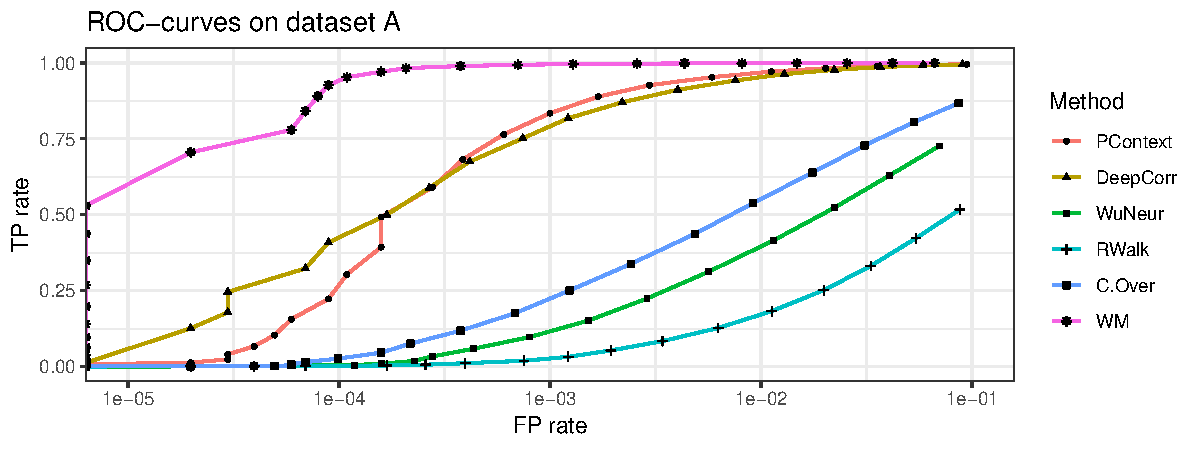
\includegraphics[width=\maxwidth]{figure/Noevasion_4nodes-1} \caption[4 nodes]{4 nodes}\label{fig:Noevasion_4nodes}
\end{figure}


\end{knitrout}

\subsection{Delays}

\begin{knitrout}
\definecolor{shadecolor}{rgb}{0.969, 0.969, 0.969}\color{fgcolor}\begin{figure}
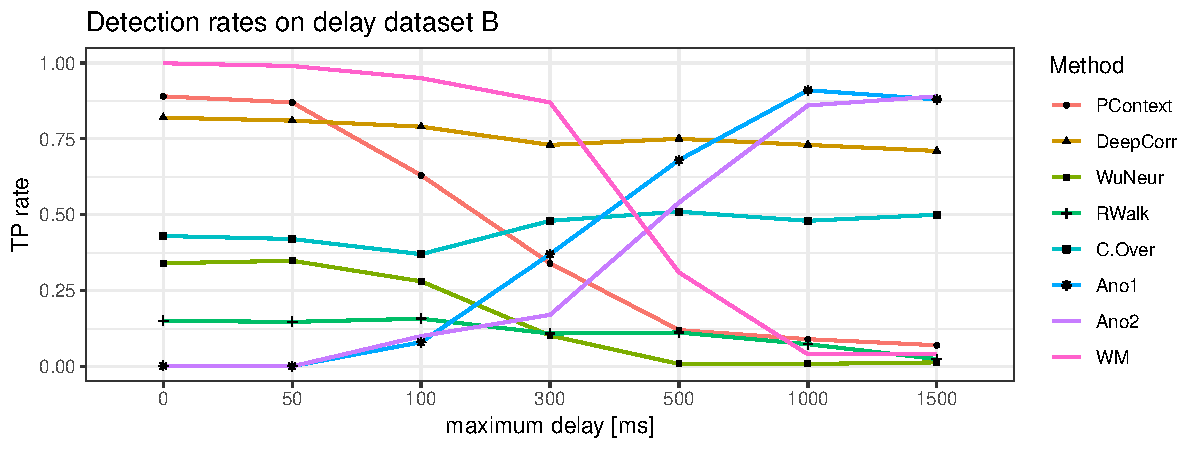
\includegraphics[width=\maxwidth]{figure/Delaydetection-1} \caption[..]{...}\label{fig:Delaydetection}
\end{figure}


\end{knitrout}


\subsection{Chaff}

\begin{knitrout}
\definecolor{shadecolor}{rgb}{0.969, 0.969, 0.969}\color{fgcolor}\begin{figure}
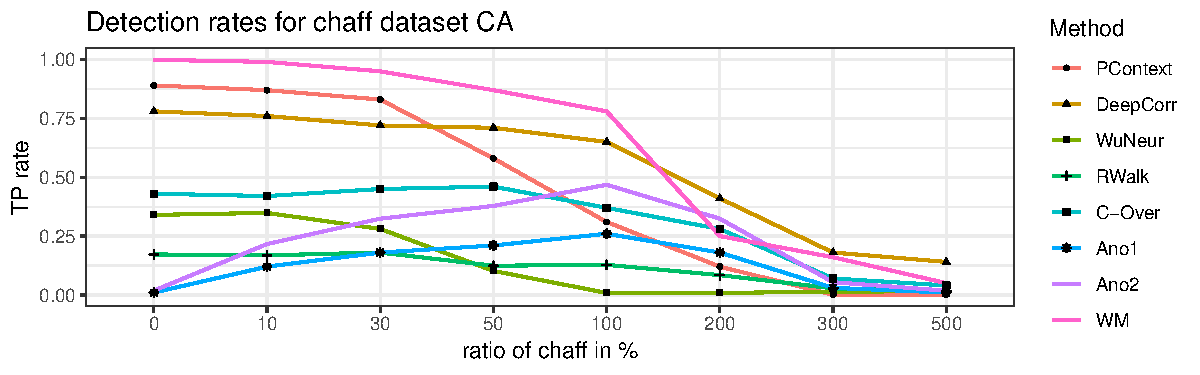
\includegraphics[width=\maxwidth]{figure/Chaffdetection-1} \caption[..]{...}\label{fig:Chaffdetection}
\end{figure}


\end{knitrout}



\subsection{Combination of delays and chaff}





\subsection{Influence of chain length on RTT-based methods}

\begin{knitrout}
\definecolor{shadecolor}{rgb}{0.969, 0.969, 0.969}\color{fgcolor}\begin{figure}
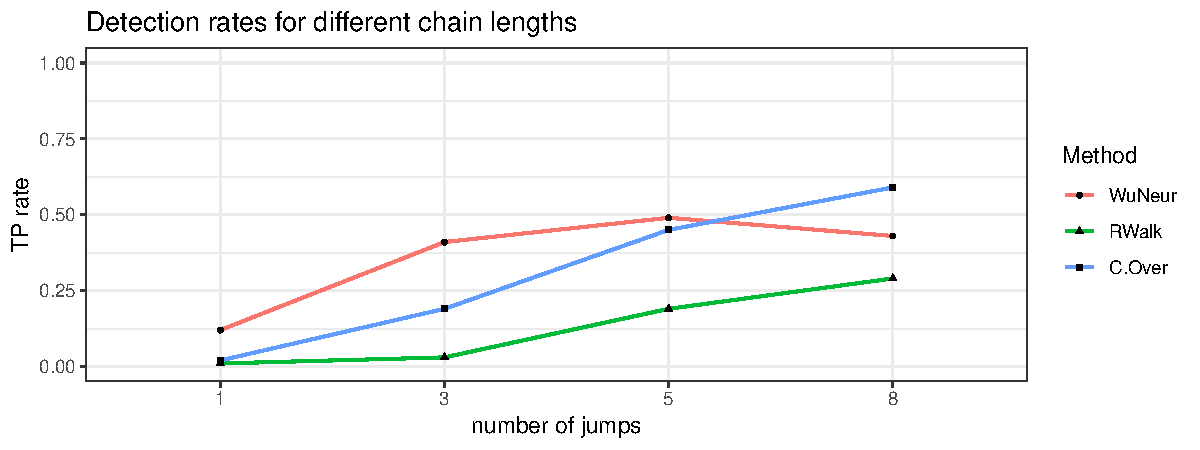
\includegraphics[width=\maxwidth]{figure/Influencechainl-1} \caption[..]{...}\label{fig:Influencechainl}
\end{figure}


\end{knitrout}


I could insert comparison of prediction accuracy on chain length


\subsection{Influence of network congestion}




\bibliographystyle{IEEEtranS}
\bibliography{NDSSrefs}

\appendix




 

\end{document}
